\chapter{OPC - UA}
Per quanto riguarda la parte di controllo, il sistema presenta un articolato insieme di controllori inter-operanti tra di loro: nello specifico ad ogni singolo controllore sono affidate delle mansioni ben specifiche, tutte ovviamente volte al controllo e alla stabilizzazione del \textit{veicolo auto bilanciato}.

In questa fase dello sviluppo del progetto, siamo andati ad implementare parte del codice che verrà installato, in un secondo momento, a bordo del raspberry: esso infatti svolge, all'interno del sistema (come si vede in figura ~\ref{fig:OPCUA_schema}) una comunicazione a due direzioni, che ne determinano due comportamenti differenti:
\begin{itemize}
	\item Come \textbf{server} per la parte di comunicazione \textit{OPC-UA} (per il settaggio dei guadagni);
	\item Come \textbf{master} nella comunicazione seriale verso Arduino (per quanto riguarda invece la gestione dell'algoritmo di controllo);
\end{itemize}

 \begin{figure}[H]
	\centering   	
	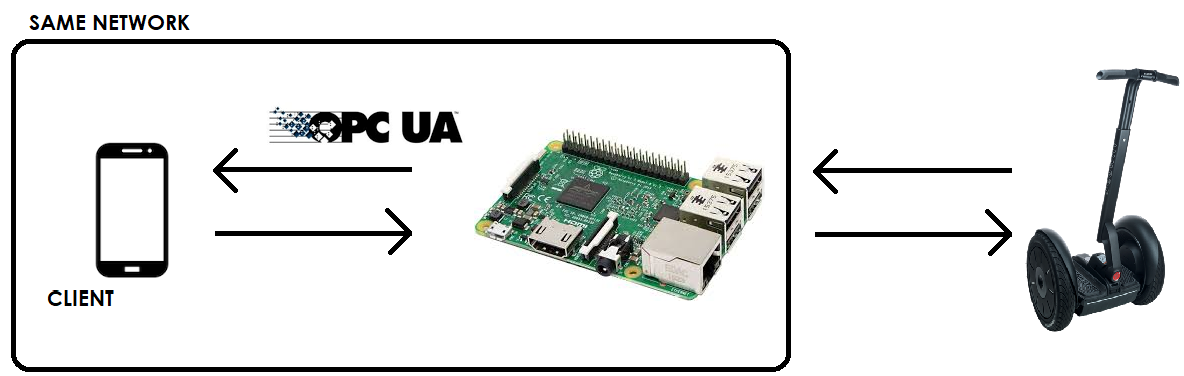
\includegraphics[width=0.75\textwidth]{Immagini/OPCUA_schema.png}
	\caption{Schema di massima dell'utilizzo di Raspberry Pi 3}
	\label{fig:OPCUA_schema}
\end{figure}

In questa fase abbiamo quindi sviluppato la parte relativa all'utilizzo di \textit{Raspberry Pi 3} come \textit{server OPCUA}.

\section{Idea base OPC-UA}
L'\textit{Open Platform Communications Unified Architecture} (OPC UA) è un protocollo di comunicazione automatico per l'automazione industriale. 

OPC UA sostituisce il protocollo \textit{OPC Classic}, conservando tutte le funzionalità del predecessore. Poiché OPC Classic era stato costruito su una tecnologia Microsoft detta modello a oggetti per componenti distribuiti, era vincolato a Microsoft, ma questa caratteristica è diventata sempre più limitante.

OPC UA risulta completamente interoperabile tra i diversi sistemi operativi usati, aggiungendosi a Windows e alle tecnologie industriali come i PLC, inoltre comprende Linux, iOS e anche sistemi operativi per dispositivi mobili come Android. Consentire al maggior numero di dispositivi possibile di comunicare contribuisce al progresso dell'IoT.

Queste caratteristiche di \textbf{interoperabilità} sono state sfruttate al massimo in questo contesto, potendo così creare, in maniera semplice e veloce, una comunicazione tra differenti tipologie e famiglie di dispositivi.

\section{OPC-UA e V.A.B.}
Nel contesto del progetto del \textit{veicolo auto bilanciato}, siamo andati ad utilizzare il protocollo di comunicazione \textit{OPC-UA} come supporto per il tuning dei parametri relativi al \textbf{gain} del controllore, ovvero ai parametri del vettore \textit{K}, che abbiamo chiamato (all'interno dello script di Python):
\begin{itemize}
	\item \textbf{K\_phi}
	\item \textbf{K\_phi\_p}
	\item \textbf{K\_theta}
	\item \textbf{K\_theta\_p}
\end{itemize}

Nello specifico, lo scambio di parametri tra server e controllore avviene tramite unfile \textit{.txt}, che permette, in maniera semplice e immediata, di implementare uno scambio di informazioni tra il server \textit{OPC-UA} strutturato in Python e l'ambiente \textit{real-time} introdotto a bordo del controllore \textit{Raspbery Pi 3}.


In particolare abbiamo due files:
\begin{itemize}
	\item \textbf{Un file temporaneo} \textit{("GainParametersToController.txt")} utilizzato come pipeline per il passaggio dei parametri tra server e controllore. Questo risulta essere un file temporaneo che viene ad essere cancellato e ricreato ogni qualvolta che il server viene spento e successivamente riaccesso.
	Nello specifico, ad ogni riaccensione, i valori iniziali di questo file, vengono settati con gli stessi valori presenti nel file \textit{definitivo}  (qualora quest'ultimo esista già: in caso contrario si procede con un inizializzazione dei parametri a 0);
	
	\item \textbf{Un file definitivo} \textit{("GainParametersConfirmed.txt")} il quale invece viene creato una e una sola volta e sul quale poi vengono salvati i parametri che saranno poi letti all'accensione successiva del server ed utilizzati come parametri iniziali per il controllore.
\end{itemize}

Questi file possono essere settati con i parametri presenti nel server che sono visibili in figura ~\ref{fig:OPCUA_params}, nello specifico:
\begin{itemize}
	\item \textbf{Submit change to controller} permette di scrivere i valori dei gains sul file \textit{"GainParametersToController.txt"};
	
	\item \textbf{Store definitively in file} permette di scrivere i valori dei gains sul file \textit{"GainParametersConfirmed.txt"};
	
	\item \textbf{SHUT DOWN SERVER} permette invece di spegnere il server e di cancellare successivamente il file temporaneo.
\end{itemize}

\begin{figure}[h]
	\centering   	
	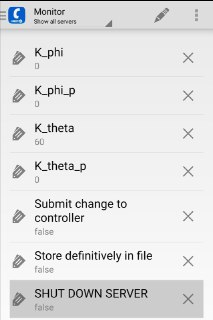
\includegraphics[width=0.4\textwidth]{Immagini/OPC_UA_params.jpg}
	\caption{Parametri impostabili lato client}
	\label{fig:OPCUA_params}
\end{figure}


Abbiamo racchiuso in figura ~\ref{fig:OPCUA_diagram} il funzionamento di massima del codice lato server: codice che siamo andati a testare utilizzando un'apposita app per smartphone Android (\href{https://play.google.com/store/apps/details?id=com.prosysopc.ua.android2&hl=it}{OPC-UA Android client}).

\begin{figure}[h]
	\centering   	
	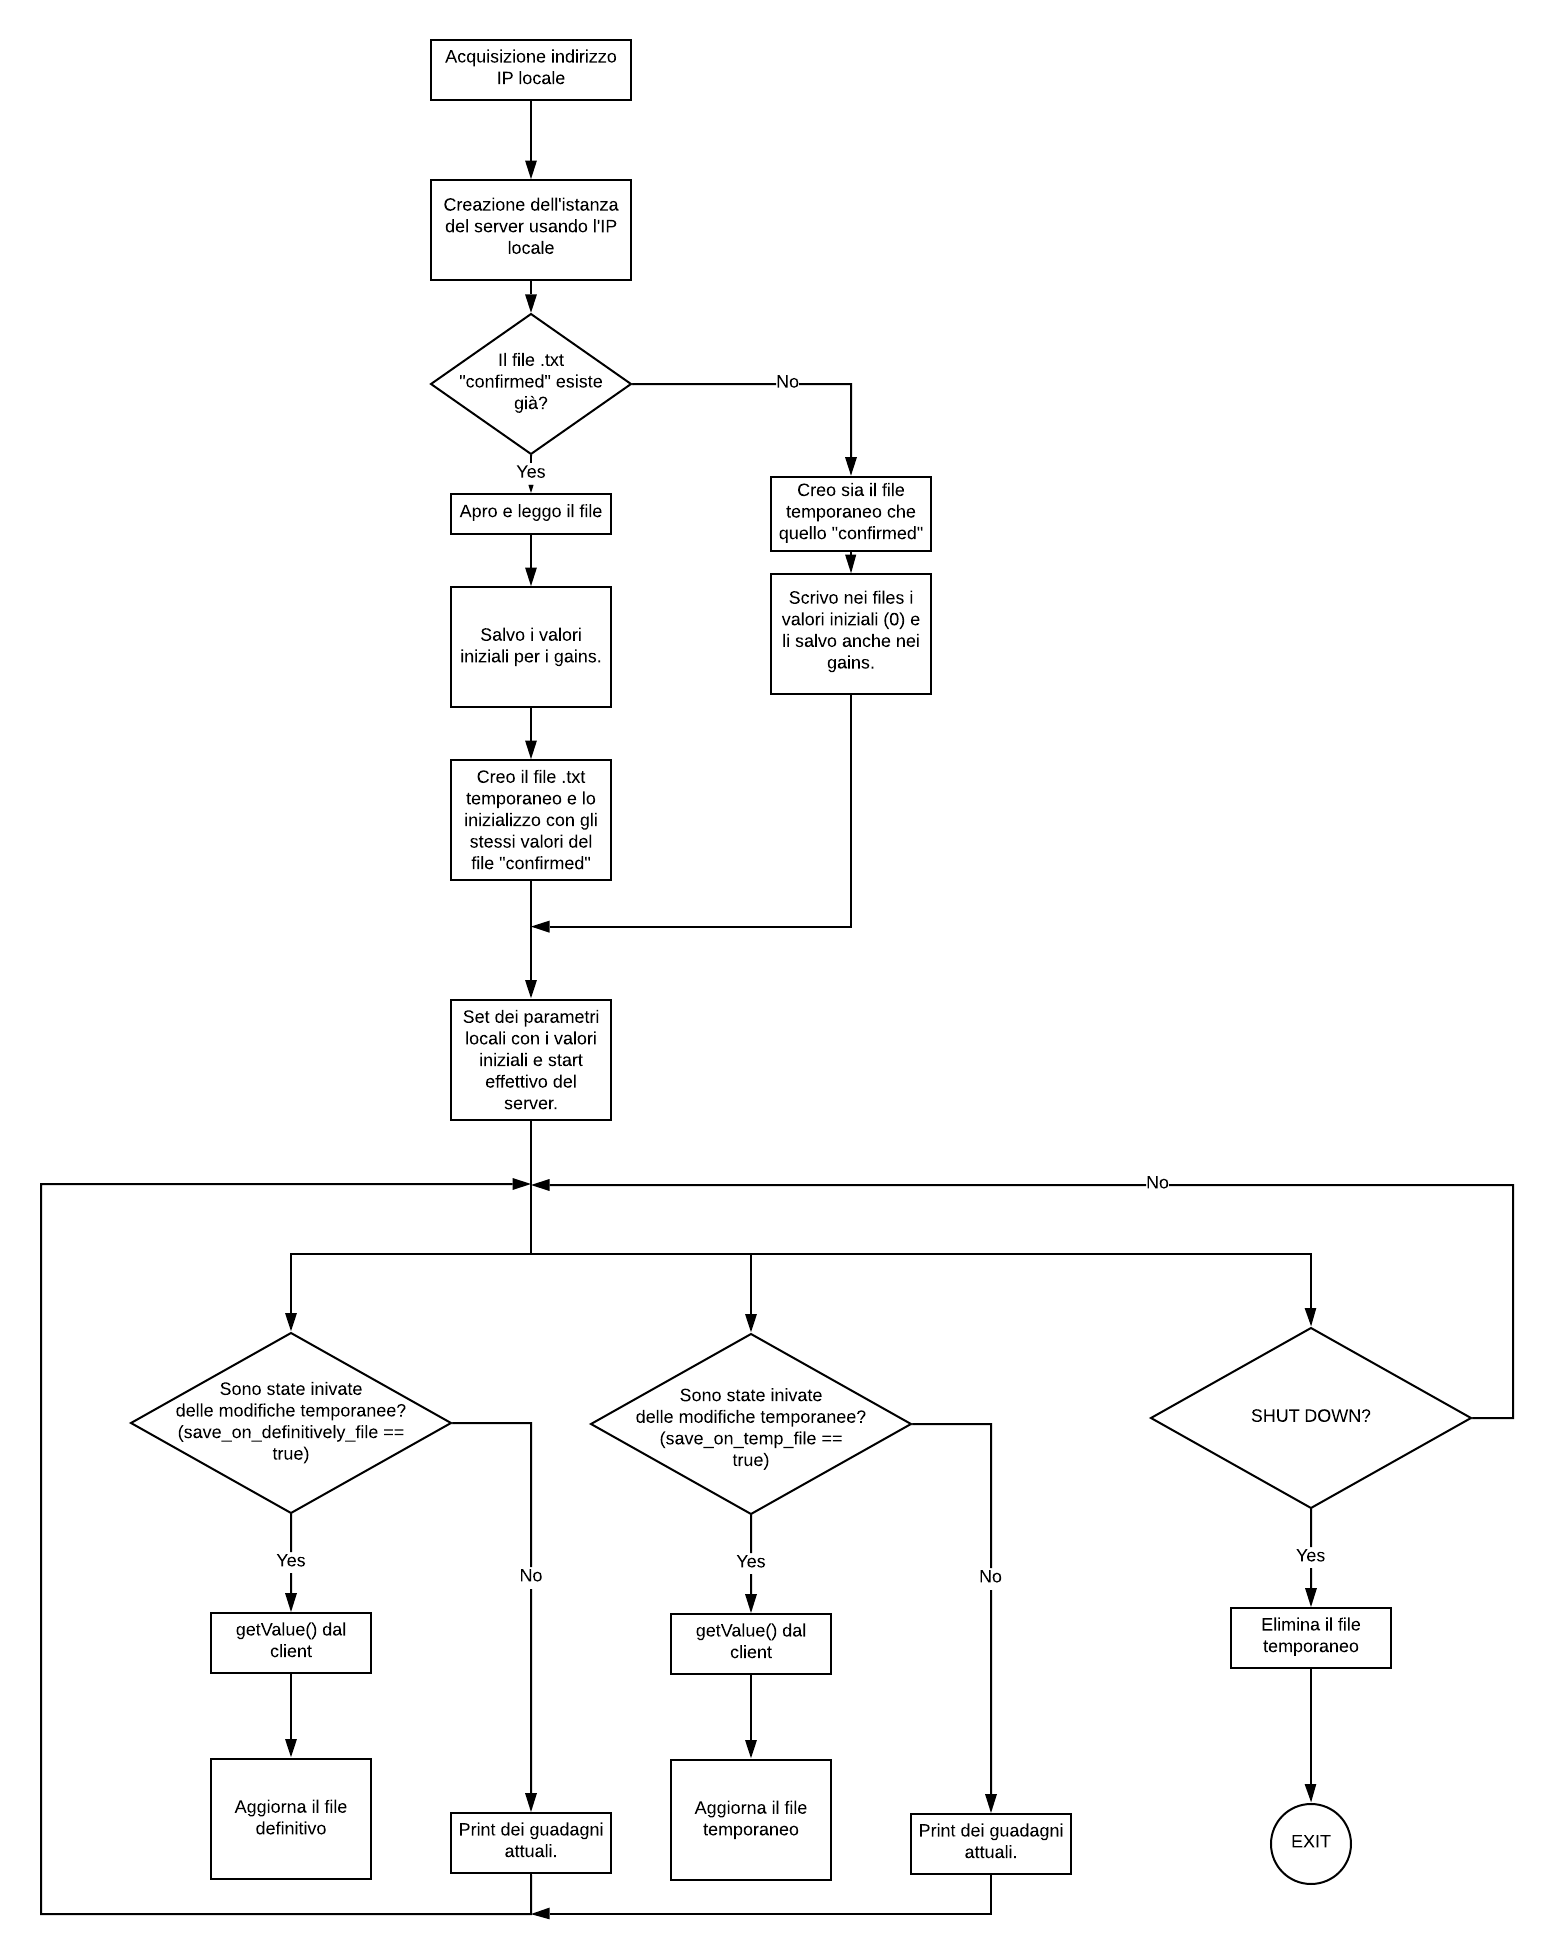
\includegraphics[width=0.7\textwidth]{Immagini/OPCUA_diagram.jpeg}
	\caption{Diagramma rappresentante le funzionalità del server}
	\label{fig:OPCUA_diagram}
\end{figure}

\chapter{Rumore}
Piattaforma inerziale --> PSD
Questione anti windup --> coppia già limitata quindi nessun vincolo di saturazione